\subsection{Retrospectives Techniques}
There are a lot of ways to perform retrospective. Around the table discussion, story-telling, weather-forecast and many more are examples of ways to conduct retrospectives. We will briefly describe two commonly used technique called KJ-session and timeline. Other techniques can be found by reading Derby and Larsen's book\cite{Larsen2006}: \textit{``Agile Retrospectives: Making Good Teams Great!''}, accessing the web page Retromat.org\cite{retromat2015} or reading our own literature review on the agile retrospective\cite{Dolvik2014}. 

\subsubsection{KJ-session}
KJ-sessions are a commonly used brainstorming technique where each participant write issues on post-it notes after the participants are done the post-it notes are grouped and discussed in the group. Dingsøyr, Moe and Nytrø\cite{Moe2001} provides an example of they conducted a KJ-session and the end-result of a KJ-session can be seen in \autoref{figure:kj-session}: 

\begin{quote}
We used a technique named after a Japanese ethnologist, Jiro
Kawakita - called the KJ-method. For each of these sessions,
we give the participants a set of post-it notes, and ask them to
write one issue on each. We usually hand out between three and
five notes per person, depending on the number of participants.
After some minutes, we ask one of them to attach one note to a
whiteboard and say why this issue was important. Then the next
person would present a note and so on until all the notes are on
the whiteboard. The notes are then grouped, and each group is
given a new name. 
\end{quote}

\begin{figure}[!h]
	\centering
	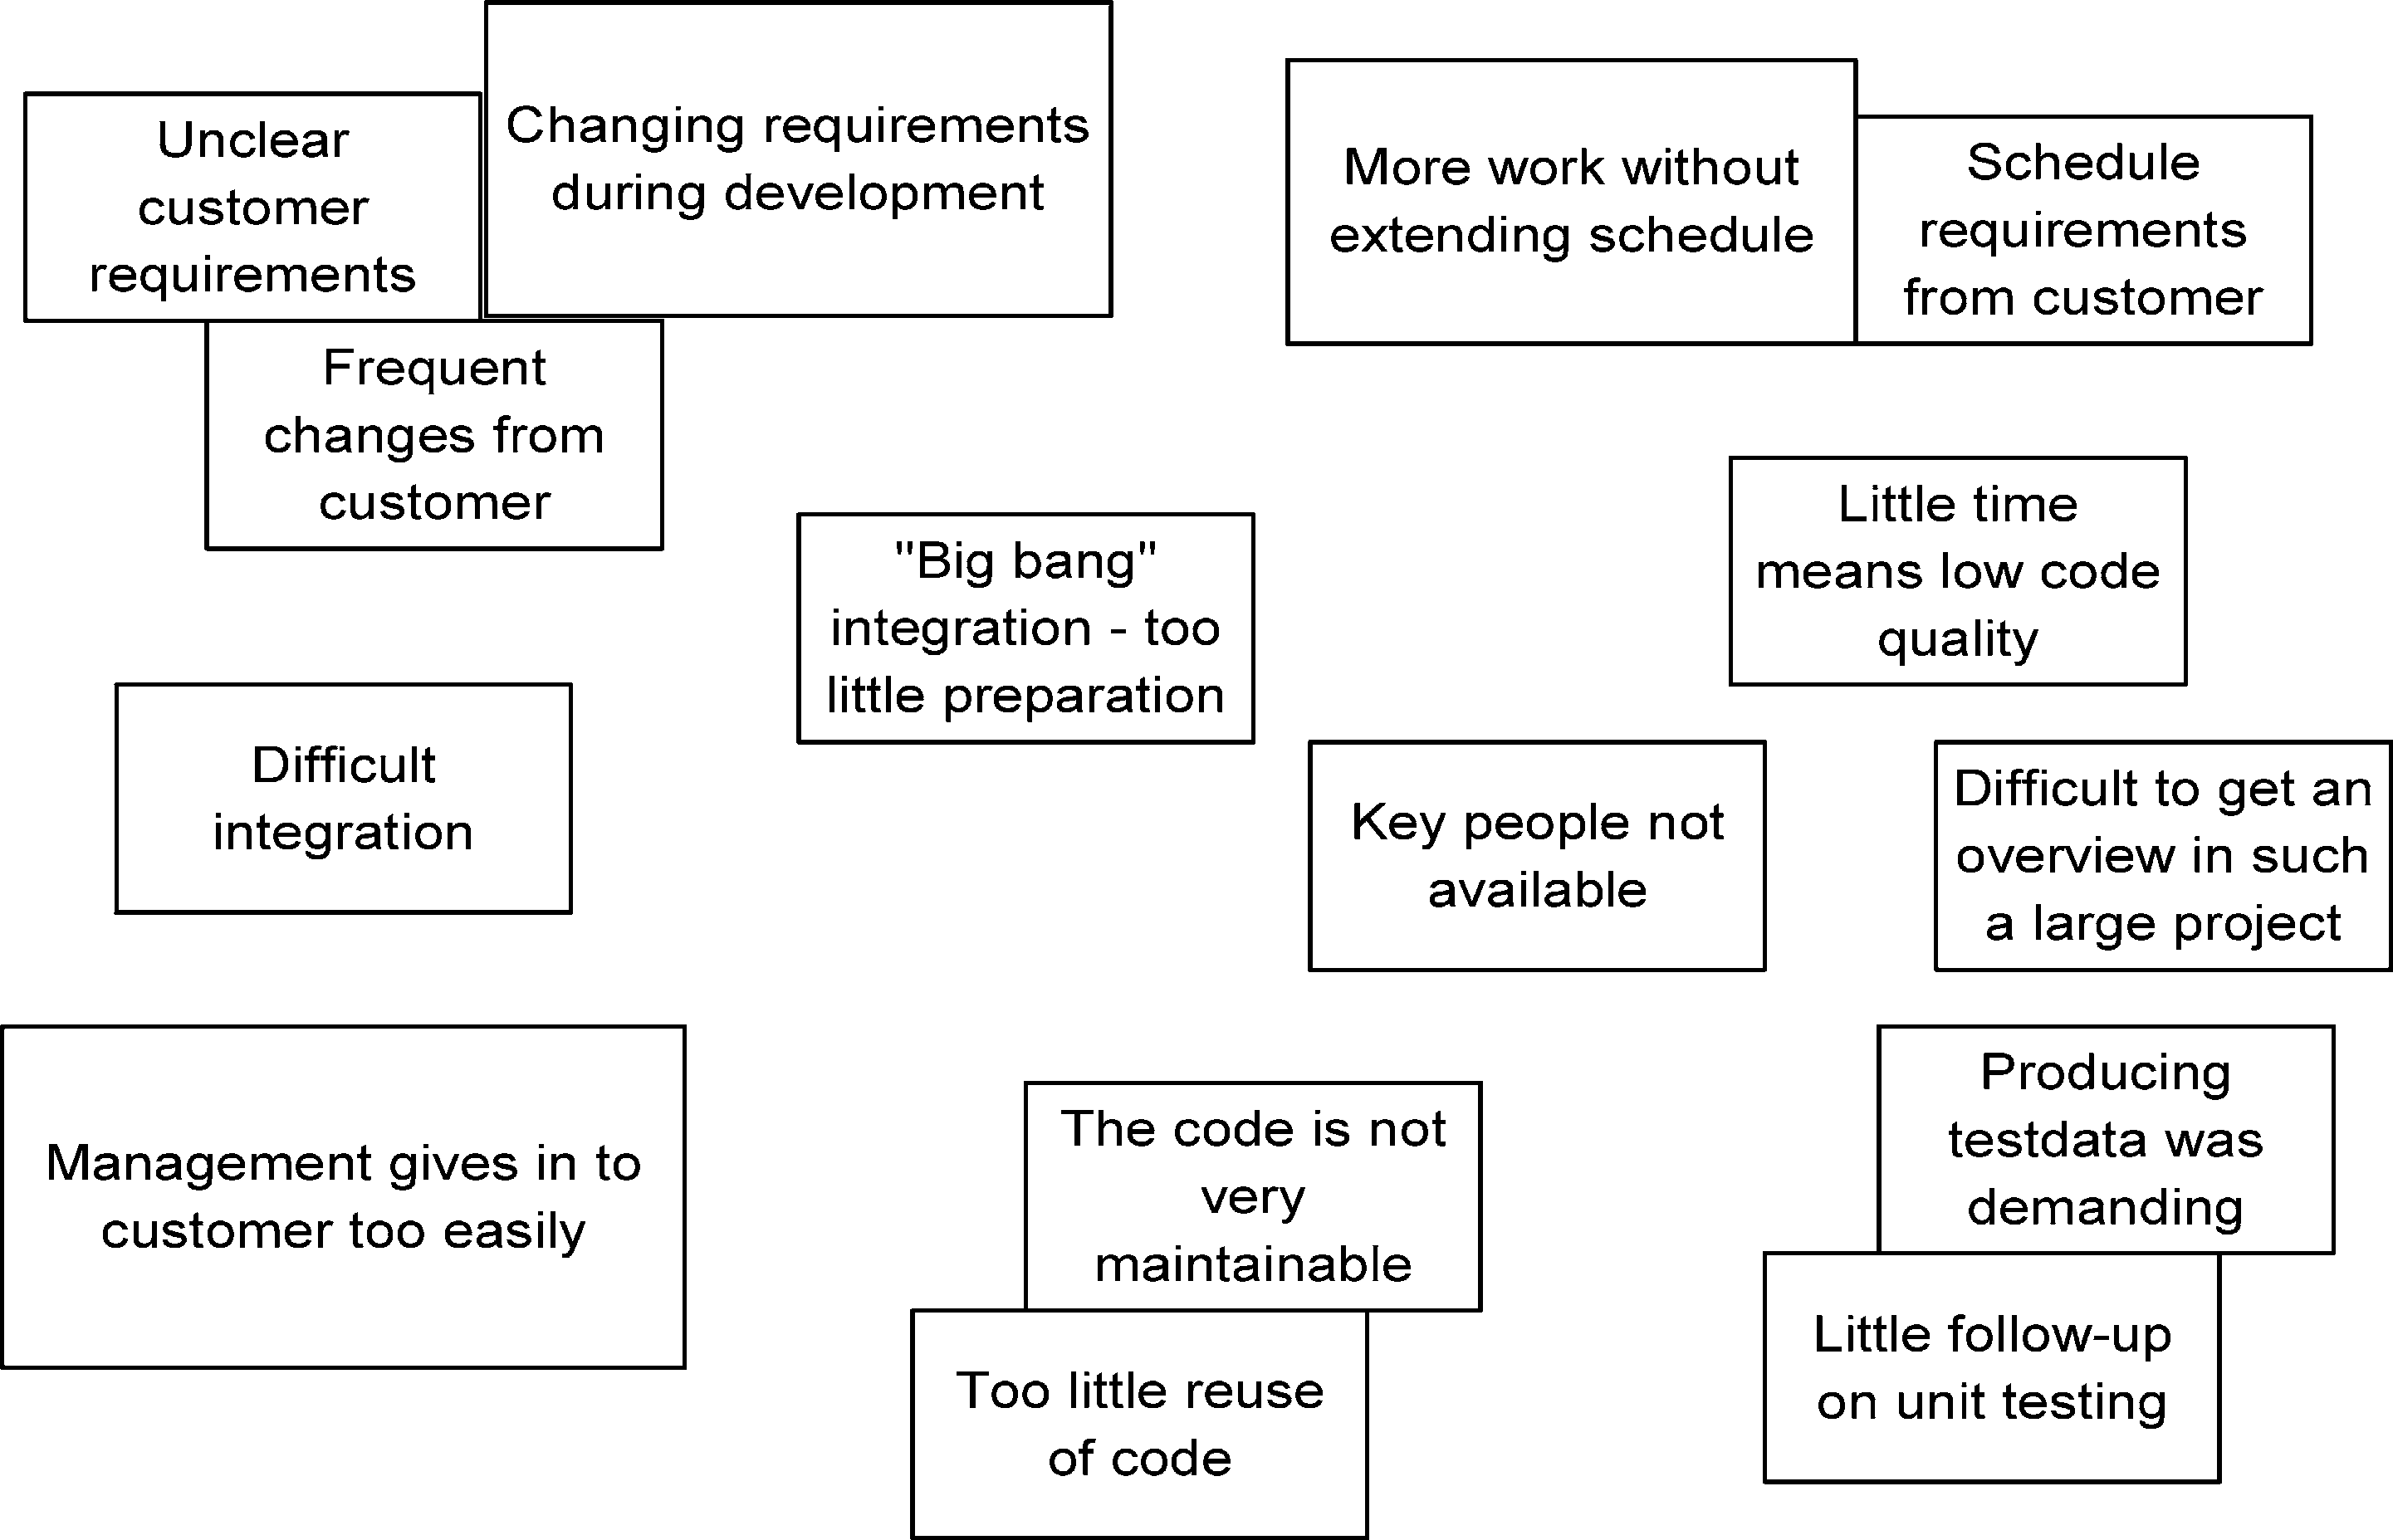
\includegraphics[width=\textwidth, keepaspectratio]{figures/KJ-session.png}
	\caption{KJ-session end result, provided by Dingsøyr\cite{Dingsoyr2004}}
	\label{figure:kj-session}
\end{figure}

\subsubsection{Timeline}
Timeline is an activity that lets the participants create a timeline over the last learning event and reflect on the event during the creation. Derby and Larsen\cite{Larsen2006} suggests that the participants should be divided into multiple groups. Each member in the group should then be handed markers and post-it notes and then write their own issues from the learning event down. Derby and Larsen suggests color-coding the post-it notes relating them to feelings, events, functions or themes. When all the participants are done writing they should together create a timeline with the post-it notes. After the timeline is done the group should analyze the timeline, looking for interesting patterns and opportunities for future improvements. An example timeline is shown in \autoref{figure:timeline}.

\begin{figure}[!h]
	\centering
	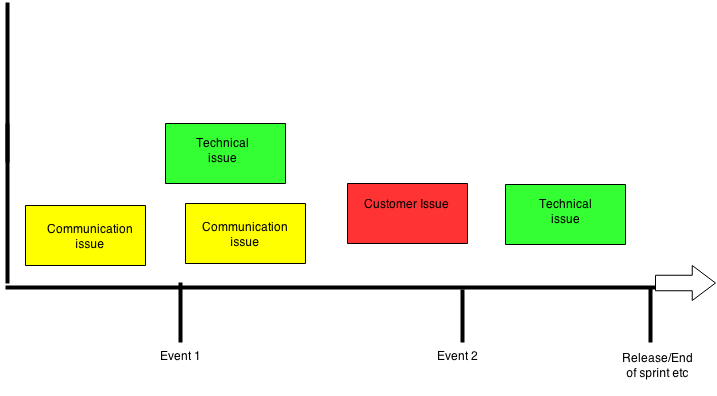
\includegraphics[width=\textwidth, keepaspectratio]{figures/Timeline-Example.png}
	\caption{Timeline illustration}
	\label{figure:timeline}
\end{figure}

There also exists a variation of timeline called; Evidence-Based Timelines, which is described by Bjarnason and Regnell\cite{Bjarnason2012}. The difference from normal timeline retropsective is that the data is collected through available systems before the retrospective. The idea is to counter bias from the participants where memory lacks and thus rather use data collected from available system during the time-period in question. A graphic example is presented by Bjarnason and Regnell and shown in \autoref{figure:e-b-timeline}. 

\begin{figure}[!h]
	\centering
	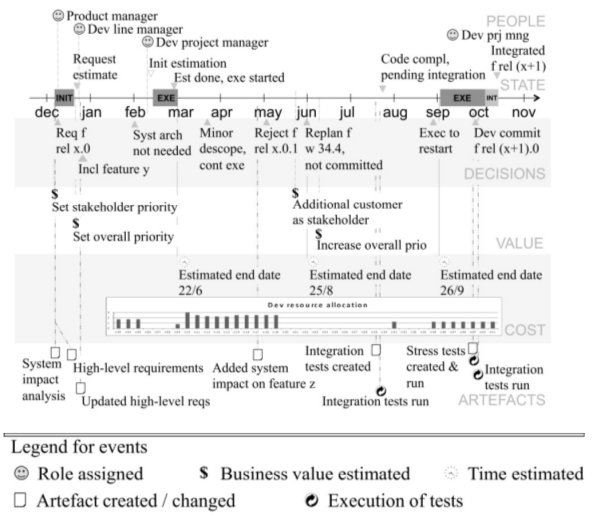
\includegraphics[width=\textwidth, keepaspectratio]{figures/eb-timeline.png}
	\caption{Evidence-based timeline illustration, presented by Bjarnason and Regnell\cite{Bjarnason2012}}
	\label{figure:e-b-timeline}
\end{figure}